\section{Modelo usando Propiedades estructurales de la Proteína}

Una de las primeras cuestiones que quisimos abordar al comienzo de este trabajo fue encontrar nuevas fuentes de información de carácter estructural de las proteínas que enriquecieran el dataset de VarQ. 

Por esta razón, una vez obtenidas nuevas variables usando ProtParam, como también las características relativas a los proteínas encontradas en SNVBox, generamos un modelo usando únicamente estos atributos con el dataset Humsavar. 


\subsection{Variables utilizadas}

\subsection{Descripción}

Las variables usadas fueron los siguientes:

\todo{TODO: Acá va una descripción de las variables}


\subsection{Correlación}

Para calcular la correlación entre las variables se usó el coeficiente de Pearson dejando únicamente aquellos valores con un p-valor inferior a 0,05.

\todo{TODO: Plot de correlación usando R}




\subsection{Resultados}

\begin{figure}[H]
    \centering
    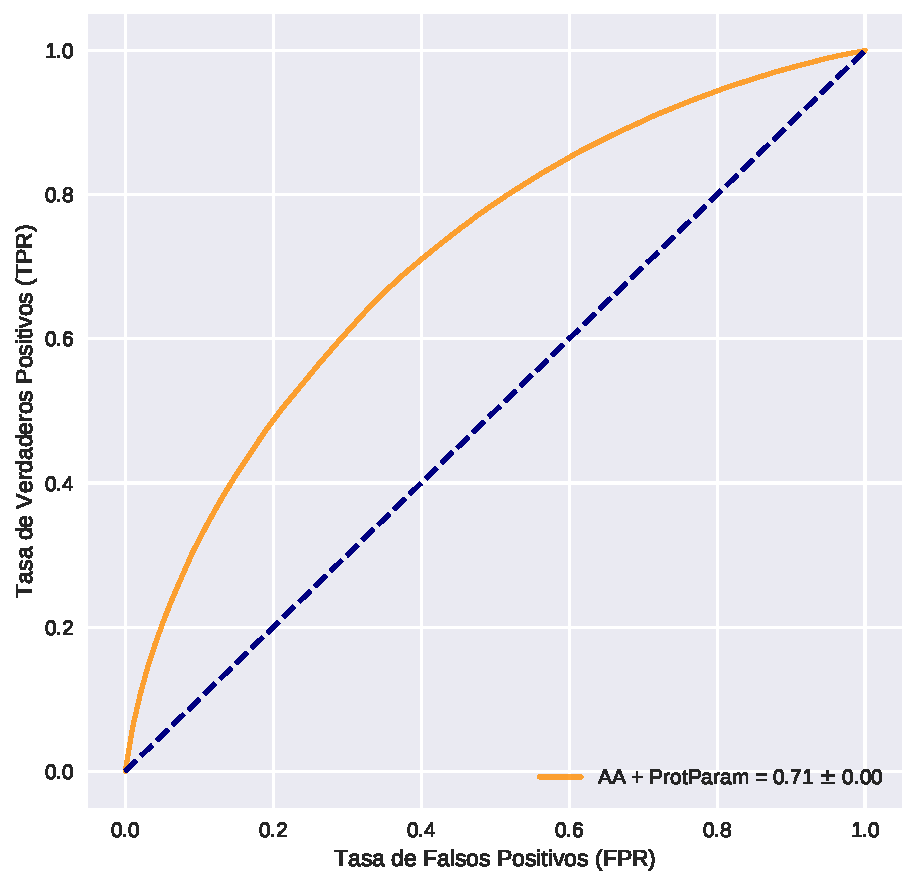
\includegraphics[scale=0.5]{documents/latex/figures/3/auc_1.pdf}
    \caption{Curva AUC del algoritmo Random Forest}
    \label{fig:auc_1}
\end{figure}


\subsection{Importancia de los atributos}

\begin{figure}[H]
    \centering
    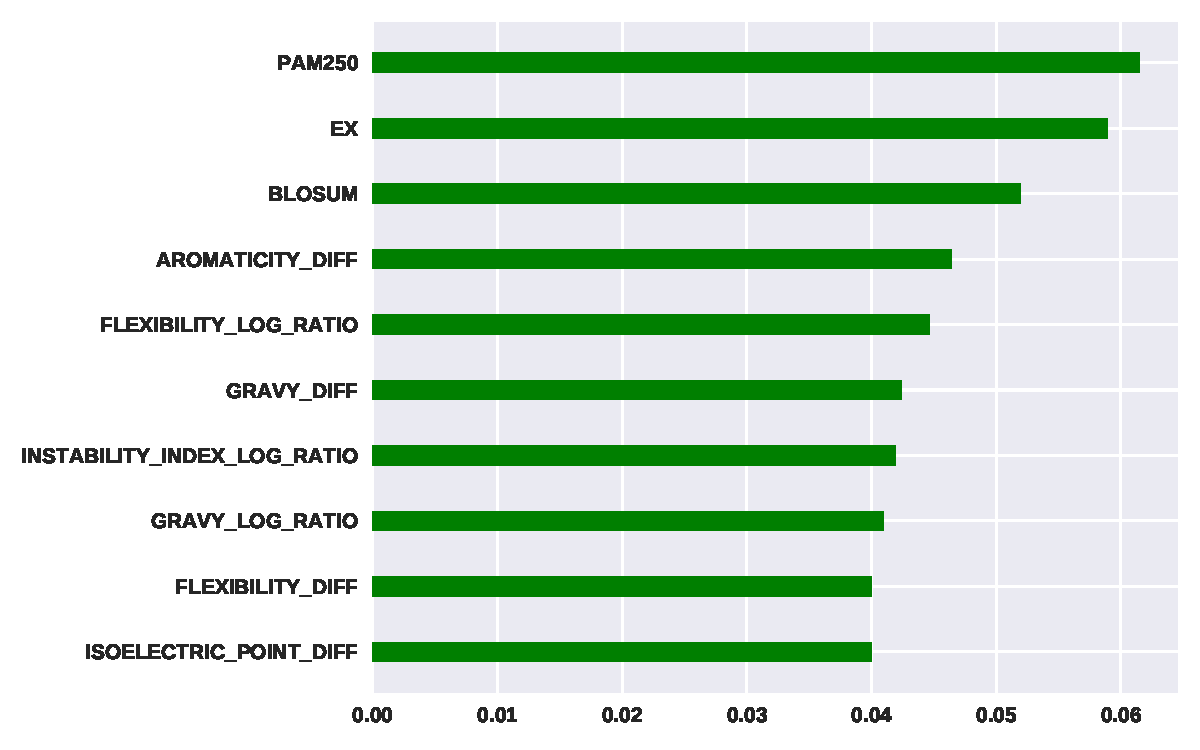
\includegraphics[scale=0.73]{documents/latex/figures/3/importance_1.pdf}
    \caption{Los 10 atributos más importantes.}
    \label{fig:importance_1}
\end{figure}


\subsection{Uniendo las variables al Dataset VarQ}

\section{Modelo usando Variables Genómicas}
\subsection{Descripción}
\subsection{Correlación}

\subsection{Resultados}

\section{Uniendo los dos Mundos}

